\section{Which bad smell could be corrected by applying the Introduce Parameter Object
refactoring?}

The bad smell which is corrected by the \textit{Introduce Parameter Object} refactoring is the \textit{Long Parameter List}. The Introduce Parameter Object groups the list of parameters  that naturally go together in an object.

\begin{center}
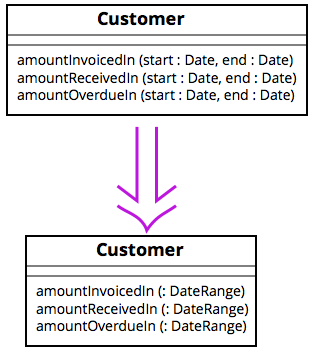
\includegraphics[scale=0.45]{LongParameterList.png}
\end{center}

\section{Which refactorings could you apply to address the Large Class bad smell?}

A large class is a class that is trying to do too much.  We can correct them with the following refactorings:

\begin{itemize}
\item  The \textit{Extract Class} refactoring : we have a class that is doing work that should be done by two. So we create a new class and move the relevant fields and methods from the old class into the new class.
\item The \textit{Extract Subclass} refactoring : we have a class that has features that are used only in some instances. So we create a subclass for that subset of features
\end{itemize}

\begin{figure}[!ht]
  \centering
  \begin{minipage}[b]{0.4\textwidth}
    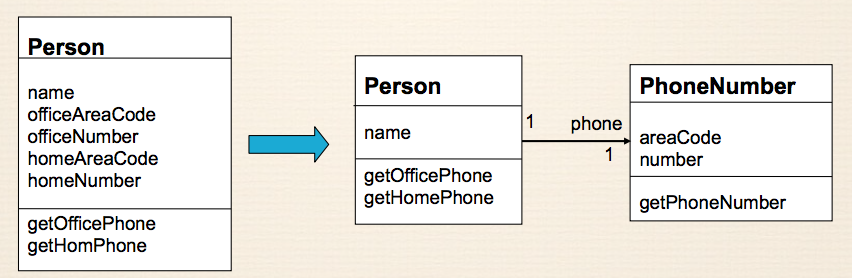
\includegraphics[width=\textwidth]{extractclass2.png}
    \caption{Extract Class}
  \end{minipage}
  \hfill
  \begin{minipage}[b]{0.4\textwidth}
    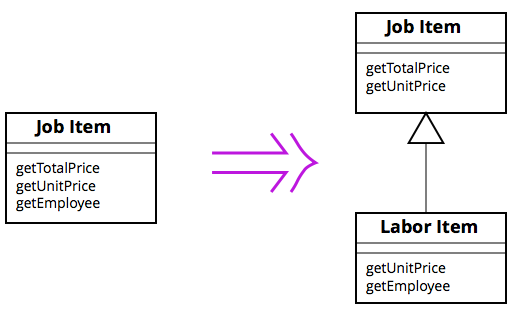
\includegraphics[width=\textwidth]{ExtractSubclass.png}
    \caption{Extract Subclass}
  \end{minipage}
\end{figure}

\section{Explain and illustrate the Long Method bad smells.}

This is a method that contains too many line of codes. And the longer a procedure is, the more difficult it is to understand what the code does. So it is :

\begin{itemize}
\item More difficult to read
\item Bad for maintainability
\item More difficult to make modifications
\end{itemize}

To avoid long methods,  we can decompose methods  in many small ones (Heuristic: whenever you feel the need to comment something, write a method instead).

\vspace{12pt}\textbf{Long method :}\\

\begin{lstlisting}
void printOwing() {
	Enumeration e = orders.elements(); 
	double outstanding = 0.0;
	// Print banner
	System.out.println("******************");
	System.out.println("***** Customer *****");
	System.out.println("******************");
    
	// Calcultate outstanding
	While (e.hasMoreElements()) {
		Order each = (Order) e.nextElement();
		outstanding += each.getAmount();
	}
	// Print details
	System.out.println("name: " + name);
	System.out.println("amount" + outstanding);
} 
\end{lstlisting} 
\vspace{12pt}\textbf{Long method corrected :}\\

\begin{lstlisting}
void printOwing() {
	printBanner();
	double outstanding = getOutstanding();
	printDetails(outstanding);
}

double getOutstanding() {...}
void printDetails(double outstanding) {...}
void printBanner() { ... }
\end{lstlisting}

\section{Same question as previous one but for one of the following bad smells:
Feature Envy or Middle Man.}

\textbf{Feature Envy :}\\
It happens when a method invokes too many times methods on another object to calculate some value (it is not logical from an OO point of view).\\
In order to correct this bad smell, we can move the method in the other class.\\

Example : \\
\begin{lstlisting}
public void mainFeatureEnvy () {
	OtherClass.getMethod1(); 
	OtherClass.getMethod2();
	OtherClass.getMethod3();
	OtherClass.getMethod4();
}
\end{lstlisting}

\vspace{12pt}\textbf{Middle Man :}\\
It happens when a class delegates to other objects and hides internal details.\\
In order to correct this bad smell, we can remove the middle man by calling directly the delegate (see lesson 5, slide 63 for further explanations).\\

Example : \\
\begin{lstlisting}
class Person{
	Department department;
	public Person getManager() {
		return department.getManager();
	}
}
class Department{
	private Person manager;
	public Department (Person manager) {
		manager = manager; 
	}
	public Person getManager() {
		return manager();
	}
}
\end{lstlisting}

\section{Explain the Long Parameter List bad smell in detail. Why is it a bad smell? How could it be
solved with a refactoring?}

The Long Parameter List means there is too much parameters for one method. It might happen after several types of algorithms are merged in a single method. A long list may have been created to control which algorithm will be run and how.\\
It is hard to understand such lists, which become contradictory and hard to use as they grow longer.\newline

We can use the \textit{Replace Parameter with Method} refactoring in order to correct it. This refactoring method says that instead of passing the value through a parameter, place the value-getting code inside the method.

\section{What’s the relation between the Long Parameter List bad smell and the Data Clumps bad
smell?}

The Data Clumps appears when different parts of the code contain identical groups of variables.\newline

As with the Long Parameter List, we can use the The Introduce Parameter Object refactoring method. The Introduce Parameter Object groups the list of parameters  that naturally go together in an object.\newline

If the data clumps are solved, it can solve the Long Parameter List in the same time because the data clumps in question may be the parameter of the Long Parameter List.

\section{Explain and illustrate what “coupling” is. Should we strive for loose coupling or tight
coupling? What bad smell describes a situation that violates this principle? Name and
explain at least one.}

Coupling is the degree to which different software components depend on each other and we should strive for \emph{loose} coupling.\newline

Tight coupling is a bad smell because it means more interdependency, more  coordination and more information flow. If we change something in a module, another module might not work anymore.\newline

A bad smell that violates this principle could be the \emph{Inappropriate Intimacy}. One class uses the internal fields and methods of another class. So it means more coupling.

\begin{center}
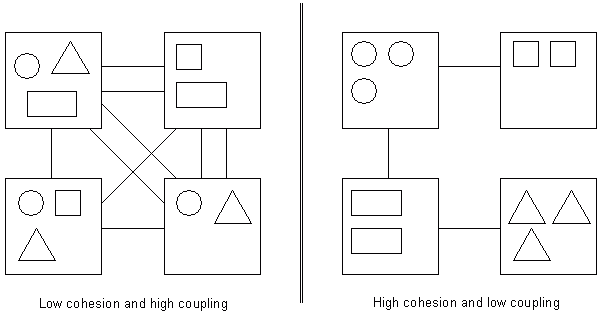
\includegraphics[scale=0.6]{CohesionCoupling.png}
\end{center}

\section{Explain and illustrate what “cohesion” is. Should we strive for low cohesion or high
cohesion? What bad smell describes a situation that violates this principle? Name and
explain at least one.}

Cohesion is the degree to which the elements within a software module belong together and we should strive for \emph{high} cohesion.\newline

Low cohesion is a bad smell because the functionalities embedded in a class have less in common and thus it is easy to lose yourself in the code.\newline

A bad smell that violates this principle could be  the Feature Envy. A method accesses the data of another object more than its own data.  So it means that the method may not belonging to the correct class.

\begin{center}
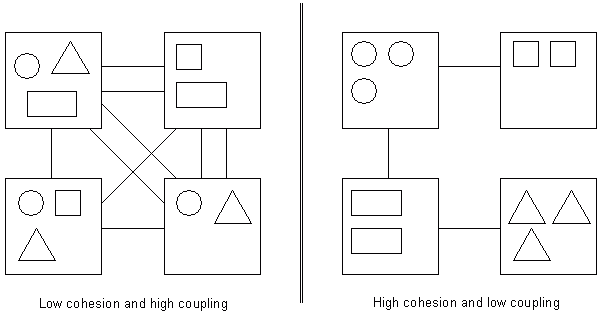
\includegraphics[scale=0.6]{CohesionCoupling.png}
\end{center}

\section{Some bad smells are based on the principle that “things that change together should go together”. Explain one such bad smell, and the above principle on which it is based, in detail.}

\textbf{Feature Envy : } when a method invokes too many times methods on another object to calculate some value, it seems more interested to put these methods into the class.

\begin{center}
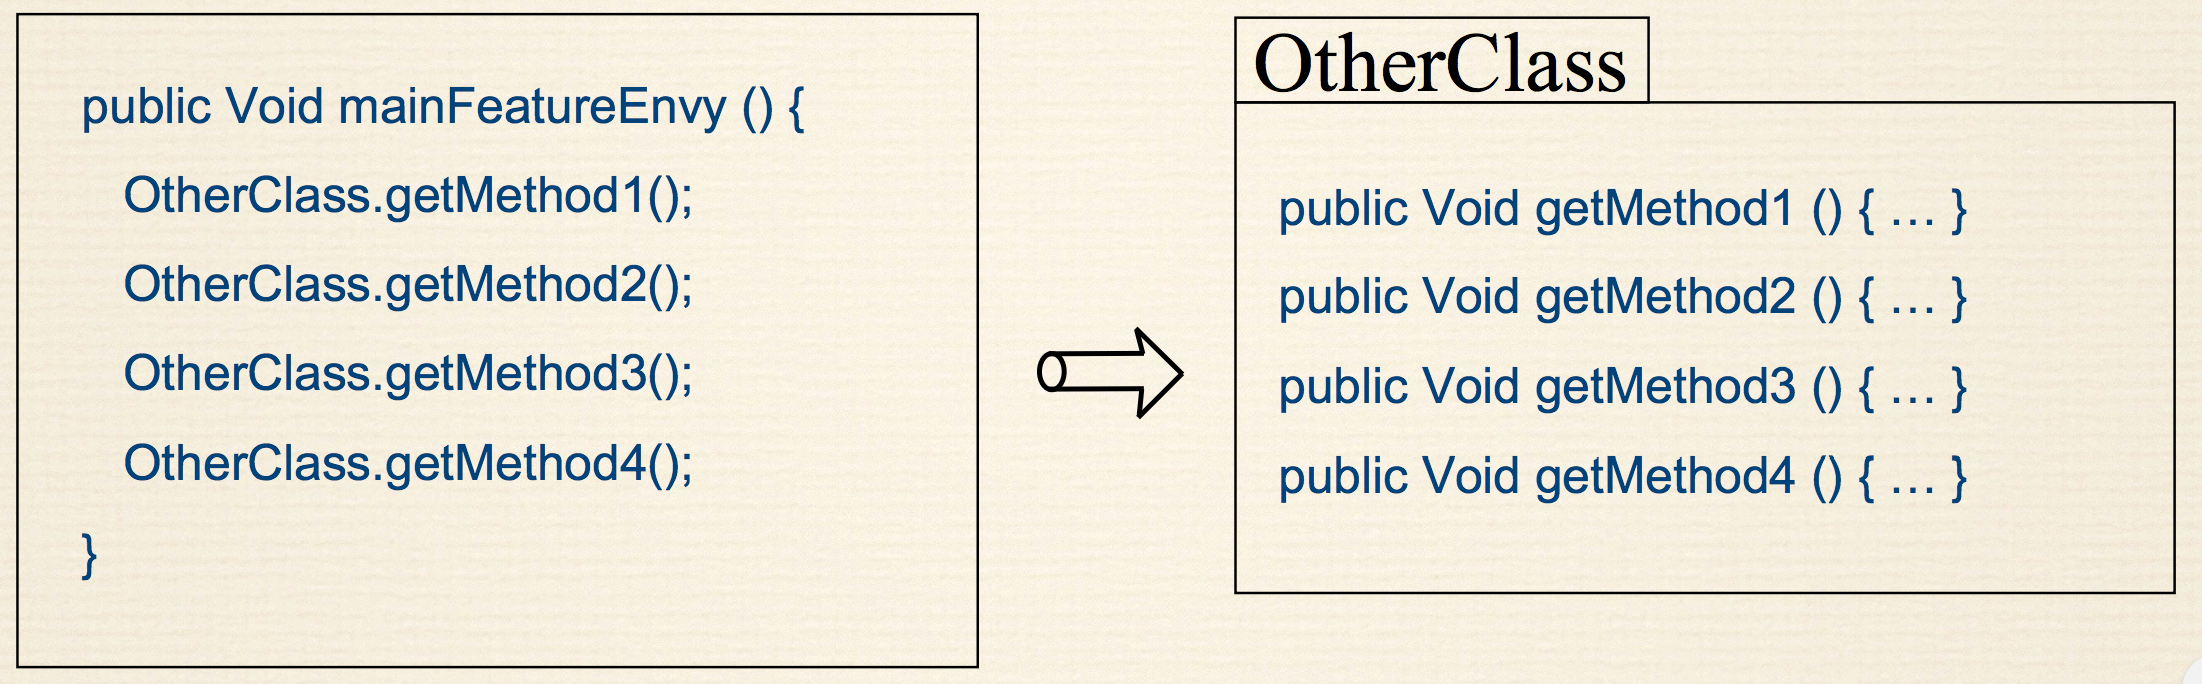
\includegraphics[scale=0.3]{feature_envy.png}
\end{center}

To resolve this bad smell, the solution is to determine which class has most of the data and put the method with that data. To refactor the code, the Move Method could be a solution and put the methods with the data.

\begin{center}
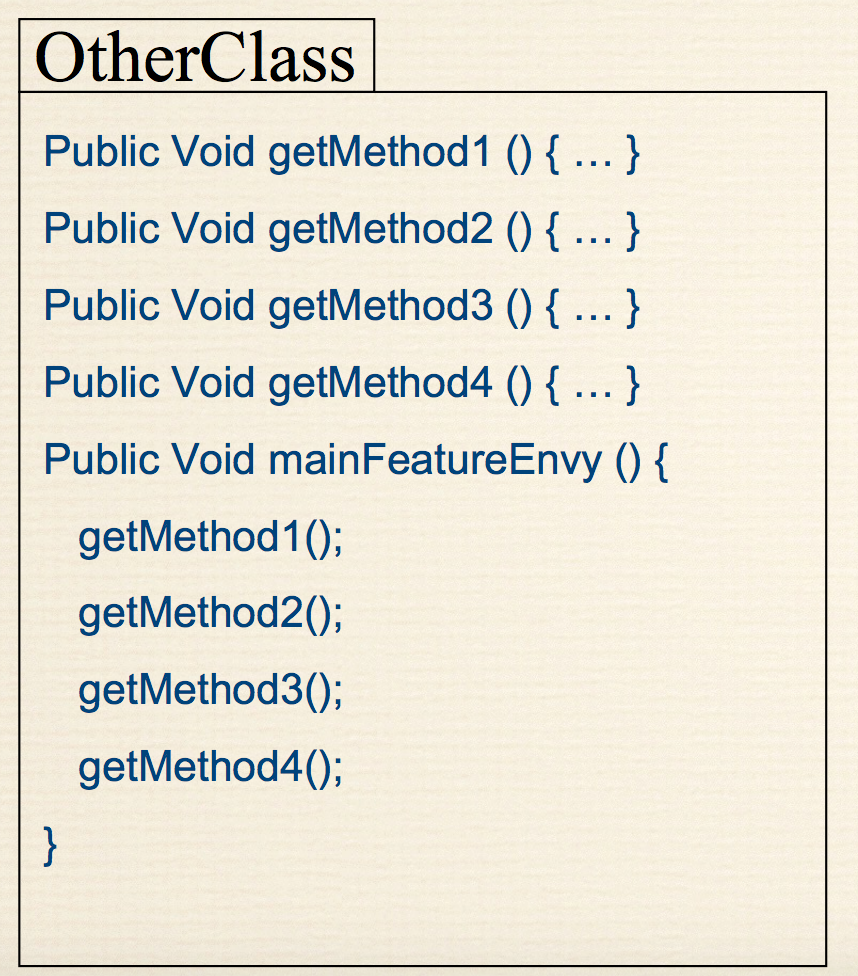
\includegraphics[scale=0.3]{feature_envy_2.png}
\end{center}



\section{Name and explain at least one bad smell that explains a problem related to bad use of inheritance.}

A problem related to bad use of inheritance could be a code duplication.

\begin{center}
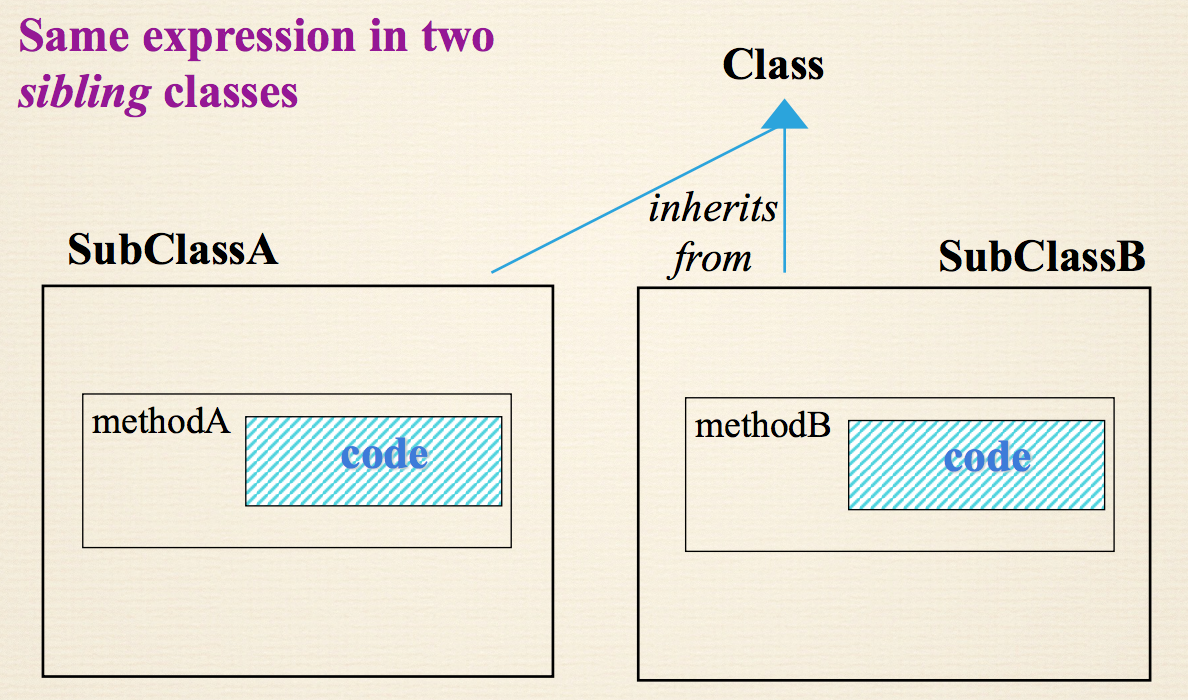
\includegraphics[scale=0.3]{inherit.png}
\end{center}

If we have same expression in two sibling classes, we have three possible cases : 

\begin{enumerate}
\item It's a \textbf{same} code : the solution is to extract method and pull up the field
\item It's a \textbf{similar} code : the solution is to extract method and use from template method
\item It's \textbf{different} algorithm : the solution is to substitute the algorithm
\end{enumerate}






\section{When talking about “Comments” in the bad smells theory session, it was stated that comments are sometimes just there because the code is bad. Can you give an example of this and how such comments could become superfluous simply by refactoring the code?}

Example : \\

\begin{lstlisting}
public double price() {
	//price is base price - quantity discount + shipping
    return quantity * itemPrice -
    Math.max(0, quantity - 500) * itemPrice * 0.05 +
    Math.min(quantity * itemPrice * 0.1, 100.0);
}
\end{lstlisting}

In general comments are good thing to have. But as we can see in the previous example, without the comment it's hard to understand what the method does. To avoid this bad smell we can use \textbf{Extract Method} and create methods whose name allows us to understand what the methods do. This problem is related to the heuristic : whenever you feel the need to comment something, write a method instead.

\begin{lstlisting}
public double price() {
	return basePrice() - quantityDiscount() + shipping();
}
public double basePrice() {
	return quantity * itemPrice;
}
public double quantityDiscount() {
	return Math.max(0, quantity - 500) * itemPrice * 0.05;
}
public double shipping() {
	Math.min(quantity * itemPrice * 0.1, 100.0);
}
\end{lstlisting}
